\section{Additional Bar charts}\label{APP:barchar}
\begin{figure}[H]
    \centering
    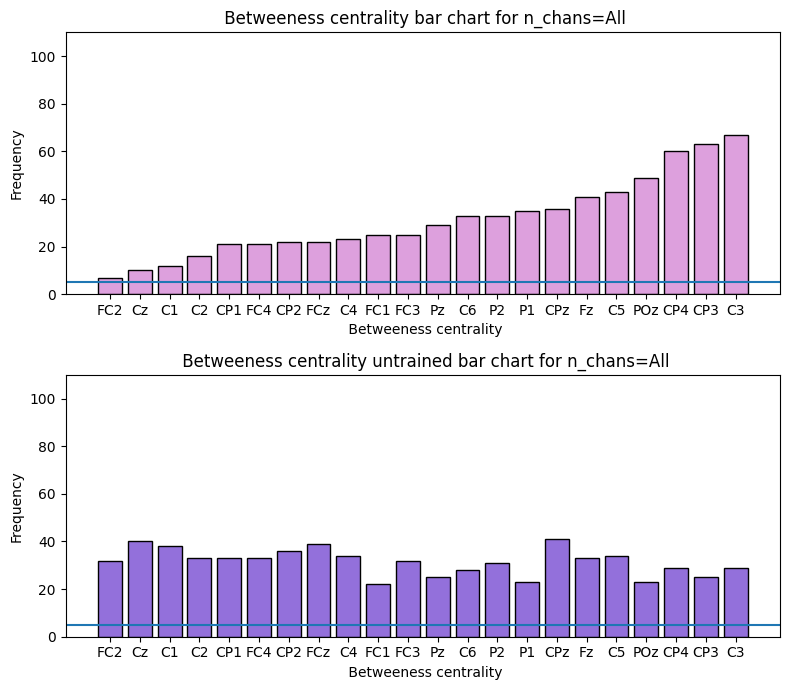
\includegraphics[width=0.75\linewidth]{img/Betweeness.png}
    \caption{Betweenness centrality bar charts for the trained (top) and untrained (bottom) models; Order of untrained bars is based on the sorted ascending order of the trained results for comparison's sake; The blue line at the frequency of 5 marks the minimal frequency requirement for the execution of a $\chi^2$ test}
    \label{fig:enter-label}
\end{figure}
\begin{figure}[H]
    \centering
    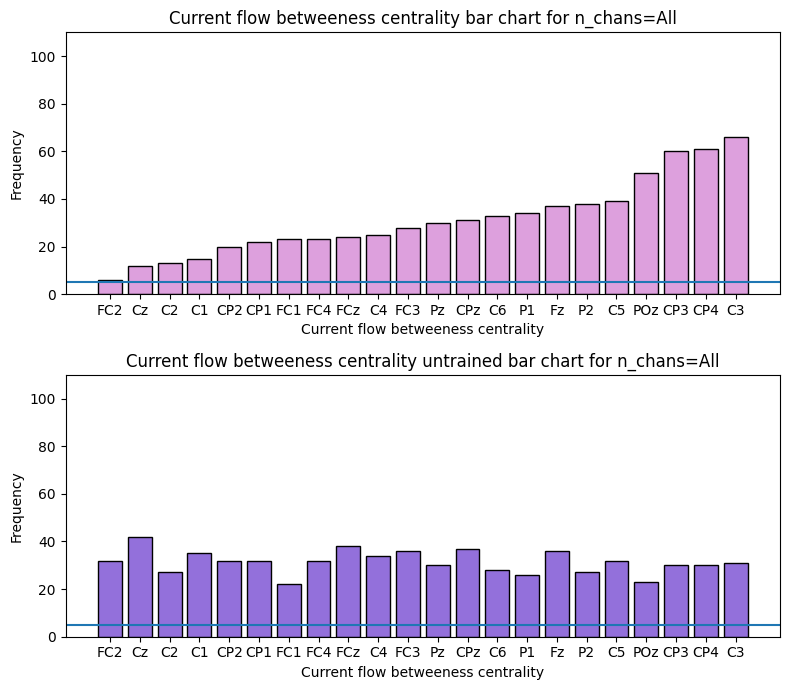
\includegraphics[width=0.75\linewidth]{img/CFB.png}
    \caption{Current-flow betweenness centrality bar charts for the trained (top) and untrained (bottom) models; Order of untrained bars is based on the sorted ascending order of the trained results for comparison's sake; The blue line at the frequency of 5 marks the minimal frequency requirement for the execution of a $\chi^2$ test}
    \label{fig:enter-label}
\end{figure}
\begin{figure}[H]
    \centering
    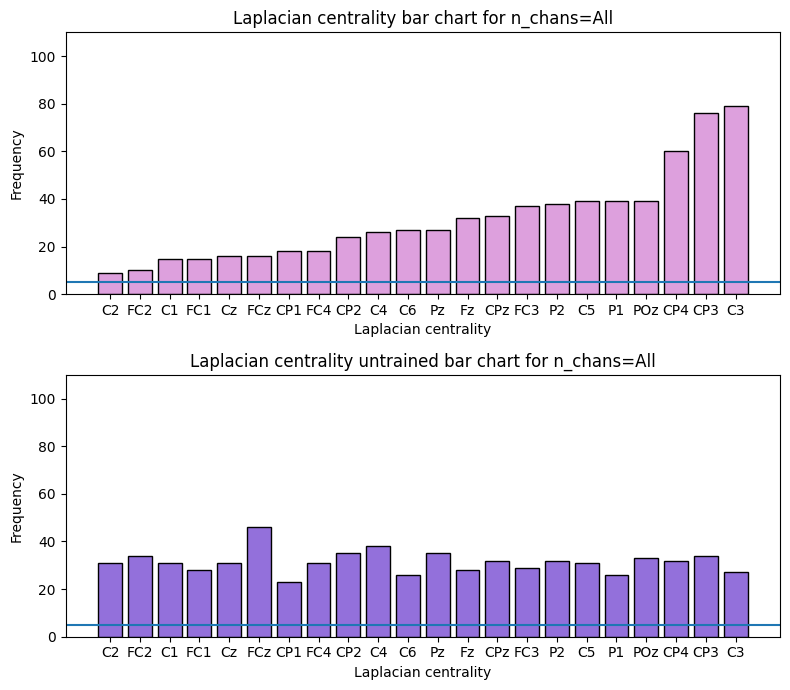
\includegraphics[width=0.75
    \linewidth]{img/Laplacianbar.png}
    \caption{Laplacian centrality bar charts for the trained (top) and untrained (bottom) models; Order of untrained bars is based on the sorted ascending order of the trained results for comparison's sake; The blue line at the frequency of 5 marks the minimal frequency requirement for the execution of a $\chi^2$ test}
    \label{fig:enter-label}
\end{figure}

\section{Full Likelihood table}\label{APP:Likelihood}

\begin{table}[H]
    \centering
    \begin{tabular}{| l | r r || r r |}
    \hline
     Node & Total & Likelihood & Above Uniform & Likelihood\\
     Label &  Trained &  Untrained & Trained  & Untrained\\        
     \hline
      CP3   & 8.97\% &  97.38\% &4.64\% &   2.02 \% \\
      C3    & 8.77\% &  92.94\% &4.74\% &   4.23 \% \\
      CP4   & 6.25\% &  37.50\% &4.44\% &  -2.42 \% \\
      POz   & 6.04\% &  33.06\% &3.73\% & -17.94 \% \\
      P1    & 5.75\% &  26.41\% &5.14\% &  13.1  \% \\
      P2    & 5.54\% &  21.98\% &4.54\% &  -0.2  \% \\
      C5    & 4.94\% &  8.67 \% &4.44\% &  -2.42 \% \\
      CPz   & 4.94\% &  8.67 \% &5.75\% &  26.41 \% \\
      Fz    & 4.94\% &  8.67 \% &4.44\% &  -2.42 \% \\
      CP2   & 4.33\% & -5.64 \% &5.14\% &  13.1  \% \\
      C6    & 4.13\% & -9.07 \% &4.23\% &  -6.85 \% \\
      Pz    & 4.13\% & -9.07 \% &4.44\% &  -2.42 \% \\
      FC3   & 3.83\% & -15.73\% &4.54\% &  -0.2  \% \\
      CP1   & 3.73\% & -17.94\% &4.33\% &  -4.64 \% \\
      FC4   & 3.73\% & -17.94\% &4.94\% &   8.67 \% \\
      C1    & 3.73\% & -17.94\% &4.74\% &   4.23 \% \\
      FCz   & 3.43\% & -24.6 \% &6.05\% &  33.06 \% \\
      FC1   & 3.33\% & -26.81\% &4.03\% & -11.29 \% \\
      C4    & 3.02\% & -33.47\% &5.24\% &  15.32 \% \\
      Cz    & 2.52\% & -44.56\% &5.75\% &  26.41 \% \\
      C2    & 2.12\% & -53.43\% &5.04\% &  10.89 \% \\
     FC2    & 1.81\% & -60.08\% &5.95\% &  30.85 \% \\     
    \hline
    \end{tabular}
    \caption{Caption}
    \label{tab:my_label}
\end{table}

\newpage
\section{All Topological maps}\label{APP:topomep}
\begin{figure}[h!]
    \centering
    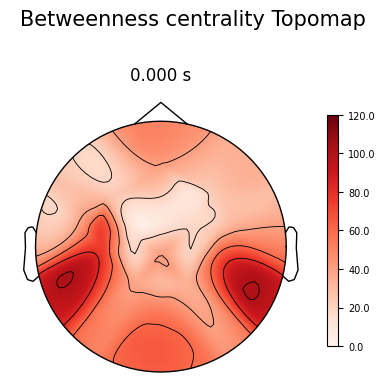
\includegraphics[width=0.55\linewidth]{img/bet_cent.png}
    \caption{Topomap of betweenness centrality frequencies of nodes; Deeper shade of red corresponds to higher node frequency}
    \label{fig:betw_cent_topo}
\end{figure}

 \begin{figure}[h]
     \centering
     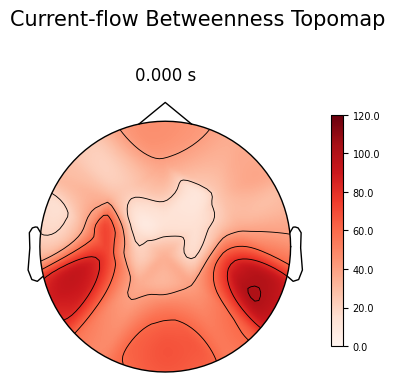
\includegraphics[width=0.55\linewidth]{img/cf_betweenness.png}
     \caption{Topomap of current-flow betweenness centrality frequencies of nodes; Deeper shade of red corresponds to higher node frequency}
     \label{fig:cf_betw_topo}
 \end{figure}

 \begin{figure}[h]
     \centering
     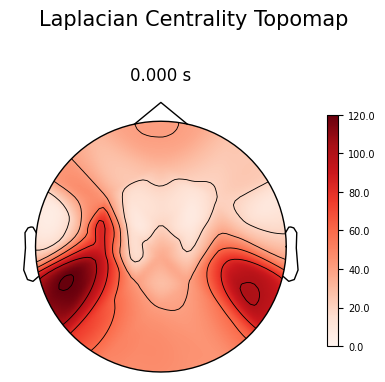
\includegraphics[width=0.55\linewidth]{img/lap_cent.png}
     \caption{Topomap of Laplacian centrality frequencies of nodes; Deeper shade of red corresponds to higher node frequency}
     \label{fig:lap_cent_topo}
 \end{figure}